\documentclass[tikz,border=10pt]{standalone}
\usepackage{tikz}
\definecolor{bg}{HTML}{171D2B}
\definecolor{accent}{HTML}{F7B538}
\definecolor{tealsoft}{HTML}{2DD4BF}
\pagecolor{bg}
\color{white}

\begin{document}
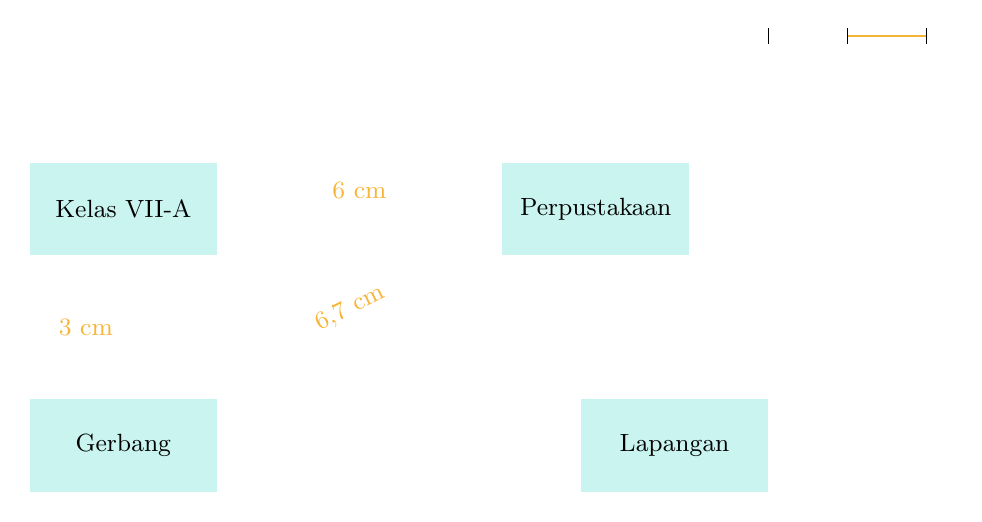
\begin{tikzpicture}[
  bangunan/.style={rectangle, draw=white, fill=tealsoft!25, thick,
    minimum width=2.4cm, minimum height=1.2cm, align=center, font=\small},
  jalan/.style={draw=white, thick},
  label/.style={font=\small\color{white}},
  jarak/.style={font=\small\color{accent}},
  scalebar/.style={font=\footnotesize\color{white}}
]

% Bangunan (koordinat dalam cm gambar; skala 1:1000 -> 1 cm = 10 m)
\node[bangunan] (gate) at (0,0)   {Gerbang};
\node[bangunan] (field) at (7,0)  {Lapangan};
\node[bangunan] (lib)   at (6,3)  {Perpustakaan};
\node[bangunan] (kelas) at (0,3)  {Kelas VII-A};

% Jalan setapak
\draw[jalan] (gate) -- (field);
\draw[jalan] (gate) -- (kelas);
\draw[jalan] (kelas) -- (lib);
\draw[jalan] (field) -- (lib);
\draw[jalan] (gate) -- (lib);

% Label jarak pada gambar (cm gambar)
\draw[jalan] (gate) -- (lib) node[midway, sloped, above, jarak] {6,7 cm};
\draw[jalan] (gate) -- (kelas) node[midway, left, jarak] {3 cm};
\draw[jalan] (kelas) -- (lib) node[midway, above, jarak] {6 cm};

% Garis skala (dua segmen 1 cm)
\draw[thick, white] (8.2,5.2) -- (9.2,5.2);
\draw[thick, accent] (9.2,5.2) -- (10.2,5.2);
\draw (8.2,5.1) -- (8.2,5.3);
\draw (9.2,5.1) -- (9.2,5.3);
\draw (10.2,5.1) -- (10.2,5.3);
\node[scalebar, below] at (8.7,5.05) {10 m};
\node[scalebar, below] at (9.7,5.05) {10 m};

% Keterangan skala
\node[label, anchor=west] at (8.2,4.4) {Skala 1 : 1.000};

\end{tikzpicture}
\end{document}
